\subsection{Follow-up diagnosis of adapter overhead}

\label{sec:adapter-ablation}

The model slowdowns motivate a controlled diagnostic rather than a claim that threshold tuning will restore an advantage. We repeat all four HF workloads on two A40s, with three independent processes per device/workload, using PyTorch 2.5.1 and Transformers 4.51.3. The two device streams run concurrently on the same host; comparisons pair policies within a process and workload. The 95\% intervals resample six device/repetition clusters over the fixed workload matrix.

Initial trials interleaved profiler sessions and subsequent policy timings within a process. A separate intervention measures the same warmed original-model decode callable in three batches before and three after a CUDA-profiler session. After/before host-time speed ratios are $0.853\times$ on GPU 0 and $0.834\times$ on GPU 1, even after the profiler context exits. These within-process batches are descriptive checks, not independent repetitions. The initial trials are retained but excluded from every final latency and candidate summary; seed 0 is remeasured in processes that never initialize the profiler. The apparent inline advantage in those initial trials is therefore not used as acceleration evidence.

All seven arms use static outer compilation with internal CUDA Graphs disabled and precision-cast emulation enabled. Decode position tensors are allocated before timing. This common configuration differs from the earlier model protocol; its ratios are not pooled with those measurements. Every arm passes eager and compiled full-logit validation for the prefill and all 64 teacher-forced decode outputs at the unchanged $10^{-2}$ tolerances. Preparation, calibration, and profiler samples are excluded from the five-warmup/20-sample prefill and two-warmup/20-sample decode measurements; event samples and a separate synchronized host batch are retained.

The archived adapter constructs an exact signature twice per call. One-lookup dispatch reuses the cached entry directly. Prebinding freezes a separately validated callable for each layer's fixed prefill/decode phase; the caller checks the phase shape and the outer compiler supplies static guards. The prebound SCIC arm reuses the corresponding legacy pre-compilation SCIC decisions, avoiding a second selection experiment. These endpoints are fixed-workload specializations, not a general dynamic-shape runtime. The static inline arm removes the outer projection--add--norm custom operation and nested compiled callable, while retaining the opaque FP16 linear boundary and cast-before-affine semantics. It contains no adaptive selector or new MemMode/ComputeMode schedule. The one-lookup implementation is promoted to the general adapter while retaining the explicit two-lookup diagnostic control.

\begin{table*}[t]

\centering\small

\caption{Follow-up adapter ablation. Each entry is a geometric mean of 24 paired host-time speed ratios. Original denotes the original compiled model under this follow-up protocol. Fixed denotes the two-lookup fixed-compiled adapter. Values below one are slowdowns.}

\label{tab:adapter-ablation}

\begin{tabular}{@{}lrrrr@{}}

\toprule

Execution path & Prefill / original & Decode / original & Prefill / fixed & Decode / fixed \\

\midrule

Fixed compiled, two lookups & 0.867 & 0.649 & 1.000 & 1.000 \\

Fixed compiled, one lookup & 0.853 & 0.670 & 0.984 & 1.032 \\

Fixed compiled, prebound & 0.904 & 0.701 & 1.043 & 1.079 \\

Inline strict, static & 0.973 & 0.897 & 1.122 & 1.382 \\

SCIC, two lookups & 0.871 & 0.647 & 1.004 & 0.996 \\

SCIC, prebound & 0.889 & 0.703 & 1.026 & 1.083 \\

\bottomrule

\end{tabular}

\end{table*}

Relative to the two-lookup fixed adapter, one lookup achieves $0.984\times$ for prefill and $1.032\times$ for decode; prebinding achieves $1.043\times$ and $1.079\times$. The prebound fixed adapter remains at $0.904\times$ and $0.701\times$ relative to the original model. Prebound SCIC reaches $0.889\times$ and $0.703\times$. Removing signature lookup alone therefore does not recover the complete-model loss. The one-lookup prefill interval relative to fixed is [0.914, 1.024]; it includes one and retains an unusually slow host batch, so no stable prefill gain is claimed.

Static strict inlining reaches $0.973\times$ (95\% interval [0.969, 0.977]) for prefill and $0.897\times$ ([0.893, 0.901]) for decode relative to the original model. This result concerns integration of a static compiled path and does not establish an adaptive-selection advantage.

\begin{figure*}[t]

\centering

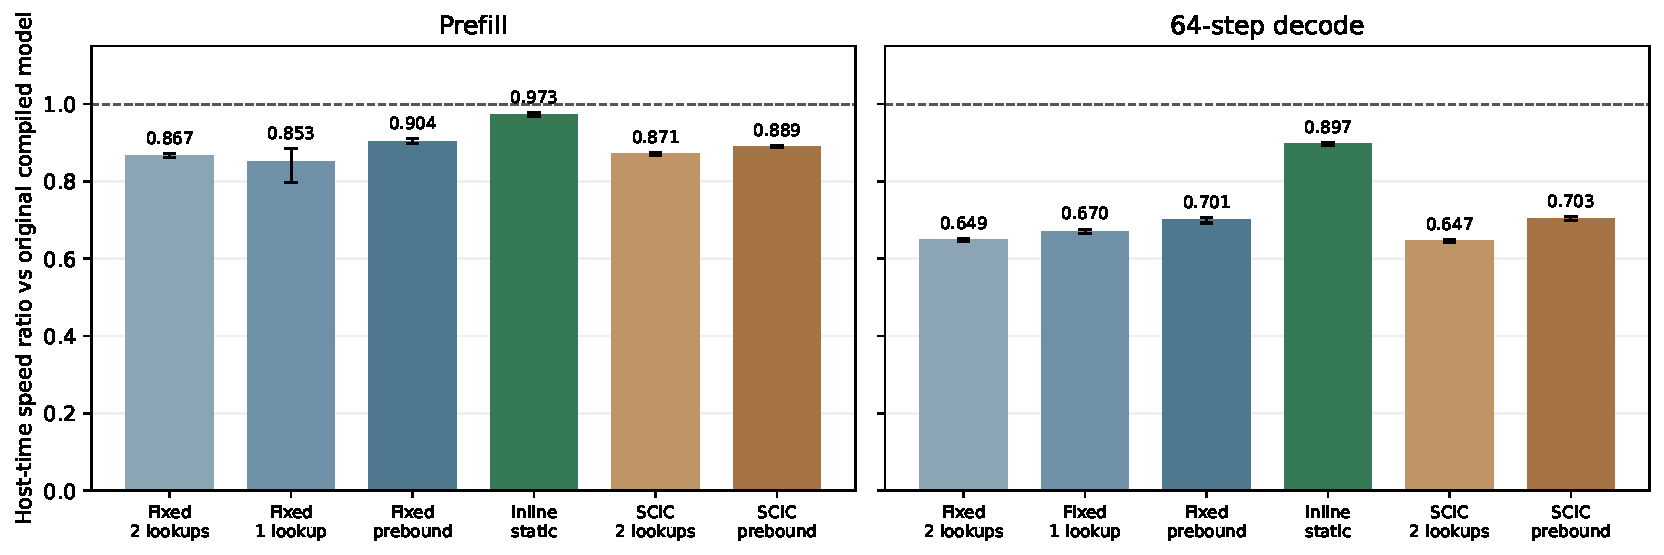
\includegraphics[width=\linewidth]{figures/fig_adapter_ablation.pdf}

\caption{Adapter diagnostics under a common follow-up protocol. Error bars resample device/repetition clusters; the original compiled model is the unit reference. Strict inlining is static, while the prebound paths specialize fixed prefill/decode signatures.}

\label{fig:adapter-ablation}

\end{figure*}

Profiler observations are retained in separate diagnostic processes; no process contributing to the final latency matrix starts a profiler. All 96 variant/workload/phase comparisons have the same CUDA-event count as their original-model reference. The opaque adapter paths enter seven compiled regions and perform seven Dynamo lookups per prefill, versus one for the original and inline paths; the 64-step decode counts are 448 versus 64. Prebinding eliminates exact-signature dispatch but retains these nested compiled calls. The archive retains CUDA-event names/counts and CPU operation counts. These are evidence about execution structure, not DRAM traffic or an isolated causal decomposition of kernel time.

A separate complete projection--residual--RMSNorm diagnostic measures six actual row counts: $M=1,8,128$ and $M=1024,2048,16384$, at width 1024 on the same six device/repetition clusters. It uses the initialized model's weight scale and unit normalization weights, preserving the $10^{-3}$ component gate. Of 36 paired shape/process measurements, native wins 25 host batches and 22 event medians. The optimistic per-shape minimum of native and compiled yields $1.155\times$ host and $1.130\times$ event speed ratios over fixed compilation. This minimum uses regular samples and is a diagnostic ceiling for this candidate set, not a measured selector or global schedule optimum. An initial arbitrary-normalization-weight smoke case failed the unchanged component gate; its rejection is retained and supplies no timing evidence for that signature.

A leave-one-seed-out check holds out both devices of each seed and selects each known shape's candidate using only event medians from the other two seeds. Its held-out ratios are $1.150\times$ for host batches and $1.127\times$ for events relative to fixed compilation; the best fixed candidate selected on training data is compiled in every fold. The held-out policy chooses native at $M=1,8,128,1024$ and compiled at $M=2048,16384$. This is offline evidence of ranking stability on known shapes, excluding dispatcher and calibration costs; it is not measured adaptive execution or unseen-shape generalization. The default analytical binding chooses compiled without probing memory-regime shapes, so it can miss the observed small-row native advantage. The crossover involves the strict adapter's existing execution paths and does not establish a transition between concrete resource-oriented kernel schedules.

The follow-up separates recoverable integration overhead from the unestablished value of analytical selection. The existing strict projection candidates have measurable local selection headroom, but adapter overhead prevents treating it as system acceleration. The next executable comparison should test all-shape empirical calibration against default SCIC and the best fixed adapter under the same invocation path. Demonstrating an intensity-guided scheduling advantage additionally requires concrete alternative schedules and evidence of the analytical feature's incremental value over empirical calibration. The diagnostic does not extend the optimized adapter to vLLM or validate pretrained normalization weights.
